\documentclass[a4paper,11pt, report]{report}

%\usepackage{UmUThesis}          % Standard English
\usepackage[noindent]{UmUThesis} % Non indented English
%\usepackage[se]{UmUThesis}      % Swedish

\usepackage[utf8]{inputenc}
\usepackage{courier}              % Nicer fonts are used. (not necessary)
\usepackage{pslatex}              % Also nicer fonts. (not necessary)
% \usepackage{lmodern}             % Optional fonts. (not necessary)

\usepackage[autostyle]{csquotes}

% \usepackage[hidelinks]{hyperref}
\usepackage{hyperref}

\usepackage{amssymb}
\usepackage{amsmath}
\usepackage{cleveref}
\usepackage{nameref}


\usepackage{csquotes}
\SetBlockThreshold{1} 


\newcommand{\mytitle}{Ranking Highscores}
\newcommand{\mysubtitle}{Evaluation of a dynamic Bucket with Global query algorithm}

\newcommand{\ra}{$\rightarrow\;$}


\hypersetup{
  bookmarks=true,         % show bookmarks bar?
    unicode=false,          % non-Latin characters in Acrobat’s bookmarks
    pdftoolbar=true,        % show Acrobat’s toolbar?
    pdfmenubar=true,        % show Acrobat’s menu?
    pdffitwindow=false,     % window fit to page when opened
    pdfstartview={FitH},    % fits the width of the page to the window
    pdftitle={\mytitle - \mysubtitle},    % title
    pdfauthor={Carl-Evert Kangas},     % author
    pdfsubject={Subject},   % subject of the document
    pdfcreator={Creator},   % creator of the document
    pdfproducer={Producer}, % producer of the document
    pdfkeywords={keyword1, key2, key3}, % list of keywords
    pdfnewwindow=true,      % links in new PDF window
    colorlinks=true,       % false: boxed links; true: colored links
    linkcolor=blue,          % color of internal links (change box color with linkbordercolor)
    citecolor=blue,        % color of links to bibliography
    filecolor=magenta,      % color of file links
    urlcolor=blue           % color of external links
}


%\usepackage{tabularx}
%\usepackage{graphicx}  

\usepackage{mdframed}

\usepackage{framed,color}
\definecolor{shadecolor}{rgb}{1.0,0.9,0.9}

\newcommand{\todo}[1] {
  \begin{shaded}
    \textbf{TODO} #1
  \end{shaded}
}

  
 
\title{\mytitle}
\subtitle{\mysubtitle}
\author{Carl-Evert Kangas}
\supervisor{Suna Bensch} 
\supervisore{}
\examiner{Juan Carlos Nieves Sanchez}
\semester{Spring semester 2016}
\course{Examensarbete, 15 hp}
\education{Kandidatprogrammet i datavetenskap, 180 hp}
\graphicspath{{img/}}  

\pagestyle{empty}

\begin{document}

\maketitle

\cleardoublepage

\begin{abstract}

  The task of ranking highscores in a computer game may sound like a trivial task. It turns out it is not, because the naive solution have a time complexity not suitable for online applications in terms of response time and running cost.

  An overview of a few approaches to ranking is presented: how an N-ary tree could be used to do ranking and how to do linear approximation. Two ways of obtaining a model for doing linear approximation are demonstrated, a method called \emph{Buckets with Global Query} is described and a method based on \emph{Frugal Streaming} is elaborated on.

  Finally, a variant of the \emph{Buckets with Global Query} algorithm where the buckets are adjusted continuosly according to the changes in the distribution of highscores is evaluated. The dynamic variant of the algorithm performs well in terms of accuracy for at least 100 000 highscore updates but have no significant gains in reduced CPU-time.

\end{abstract}

\vskip2\baselineskip
\vspace{5mm}
\begin{center}
  {\Large\bfseries Att ranka rekord \\ \vspace{3mm}
    \small En utvärdering av en dynamisk implementation\\av algoritmen \emph{Buckets with Global Query}}
\end{center}

\begin{abstract}[Sammanfattning]

  
  Den naiva lösningen till att ranka ett rekord i ett spel är att räkna antalet rekord som är bättre än det rekord man har för handen. Lösningen skalar inte då den har en tidskomplexitet på $\mathcal{O}(n)$ och kan därför inte användas i ett onlinespel då responstiden skulle bli för lång och kostnaden för hög.

  En överblick över några sätt att angripa problemet presenteras; hur man kan lösa problemet med hjälp av ett träd samt tillvägagångssätt som bygger på linjär approximation. Två sätt att ta göra rankning med linjär approximation demonstreras. \emph{Buckets with Global Query} är en algoritm som bygger en modell av distributionen av alla rekord med jämna mellanrum. En alternativ lösning som bygger på en algoritm för att ta fram kvantiler ur en dataström presenteras.

  Slutligen utvärderas en variant av \emph{Buckets with Global Query} där modellen som approximationerna görs ifrån kontinuerligt uppdateras för att motsvara den verkliga distributionen av alla rekord. Den dynamiska varianten av algoritmen har god precision men är inte nämnvärt effektivare än den ursprungliga.

\end{abstract}

\cleardoublepage

\chapter*{Acknowledgements}

I would like to thank my supervisor Suna Bensch for all support and feedback during the writing of this thesis.

Special thanks to my partner Peter Sundqvist for moral as well as technical support during this project.

\cleardoublepage
 
 
 
\tableofcontents
\cleardoublepage

\pagestyle{fancy}
\setcounter{page}{1}

\chapter{Introduction}

\section{Background}

\begin{shaded}
  Define ranking. Citation from Wikipedia, need better source.
\end{shaded}
``A ranking is a relationship between a set of items such that, for any two items, the first is either 'ranked higher than', 'ranked lower than' or 'ranked equal to' the second''

\begin{shaded}
  Typical CS related ranking scenarios - AI, search engines
\end{shaded}
 



\begin{shaded}
  Scoring function - How to produce ordinal numbers 
\end{shaded}

\subsection{Ranking in online games}

\begin{shaded}
Define what ranking is in the context of games. Ie what to rank time or skills? In case of skills - same skills may not translate into same score (as in TrueSkill). 

\end{shaded}

\textbf{Determine winning player or creating a leaderboard}

Most games have some kind of skill based ranking system in order to make the game interesting. Usually the skills are expressed as a score, ie a number.


Higher score \ra better

TrueSkill (scoring function) \ra score

time \ra lower or higher time is better

\textbf{Matching players}
The score that players get in a game may also be used to determine winners of tournaments, for gambling, for pairing similarily skilled players in a matchmaking process and so on.

\textbf{Approximate ranks are OK in many cases} Approximate matches of queries are commonplace in the text world (Top-k Selection Queries over Relational
Databases: Mapping Strategies and
Performance Evaluation)

General requirements (ie. an exact solution may not be needed all the time - may be crucial among the highest scores, when competing and if there is some gambling.
  
\section{Problem description}

\begin{shaded}The goal with this section is to

  1) clearify why this seemingly trivial problem is a real problem (O(n) \ra not feasible

  2) Something about a a very common business model (small startup, free-to-play) limited budget and business not large enough to run server park on its own. \end{shaded}

How to get a live rank for a score when set of scores are large

\subsection{Infrastructure}

\begin{shaded}
  Running applications on Platform-as-a-Service-services have implications on the application to be run.

  Performance-related-issues, cogestion.

  Pricing.

  \end{shaded}

Google App Engine (often referred to as GAE or simply App Engine) is a platform as a service (PaaS) cloud computing platform for developing and hosting web applications in Google-managed data centers. Applications are sandboxed and run across multiple servers.

Java, other languages
 
Other services (memory cache)

\textbf{App Engine Datastore} is a schemaless NoSQL datastore providing robust, scalable storage for your web application.

\subsubsection{Pricing}

Price model

\chapter{\label{method}Method}

The question to be researched is whether an adaptive bucket-table can be made to do ranking more efficient than a static table with offline updates.

\section{Problem description revisited}

The Companys current ranking algorithm is an implementation of the algorithm \emph{Bucket with Global Query} (See \labelcref{bucket}). The highscores are stored in Google App Engines Datastore as entities with properties \emph{username} and a \emph{highscore}. When a player gets a new highscore it replaces the old highscore.

Since score in this case is measured in milliseconds and lower timings are better a better score is a lower number\footnote{While this really should not matter at all, be aware that this fact is a good foundation for getting mindfucked very hard}.

A background job  periodically iterates through all the highscores making the bucket-table that contains ranks and scores needed to make the estimates. The entities are indexed on highscore-property which is essential to make the process of iterating through the whole set doable.

\section{Hypothesis} 

The current implementation starts a background job that builds the bucket-table every ten minutes. When the scan is complete a reference is set to the new table and the old one is discarded. The accumulated error is at its maximum right before the switch and will in the forthcoming reasonings serve as an upper limit for what would be an acceptable performance.

The total cost for providing the ranking service with the current implementation and the implementation to be assessed is $n \times costforestimate + \frac{ costfortablecreation}{n}$.

\todo{Better formula}

The hypothesis is as follows:

\blockquote{Running the ranking service with the new implementation will be more efficient than the current implementation at the same level of error.}

\begin{figure}[h]
  \centering
  \caption{Cost vs time. Dotted line is the outcome when hypothesis the hypothesis is true.}
  \label{fig:cost}
  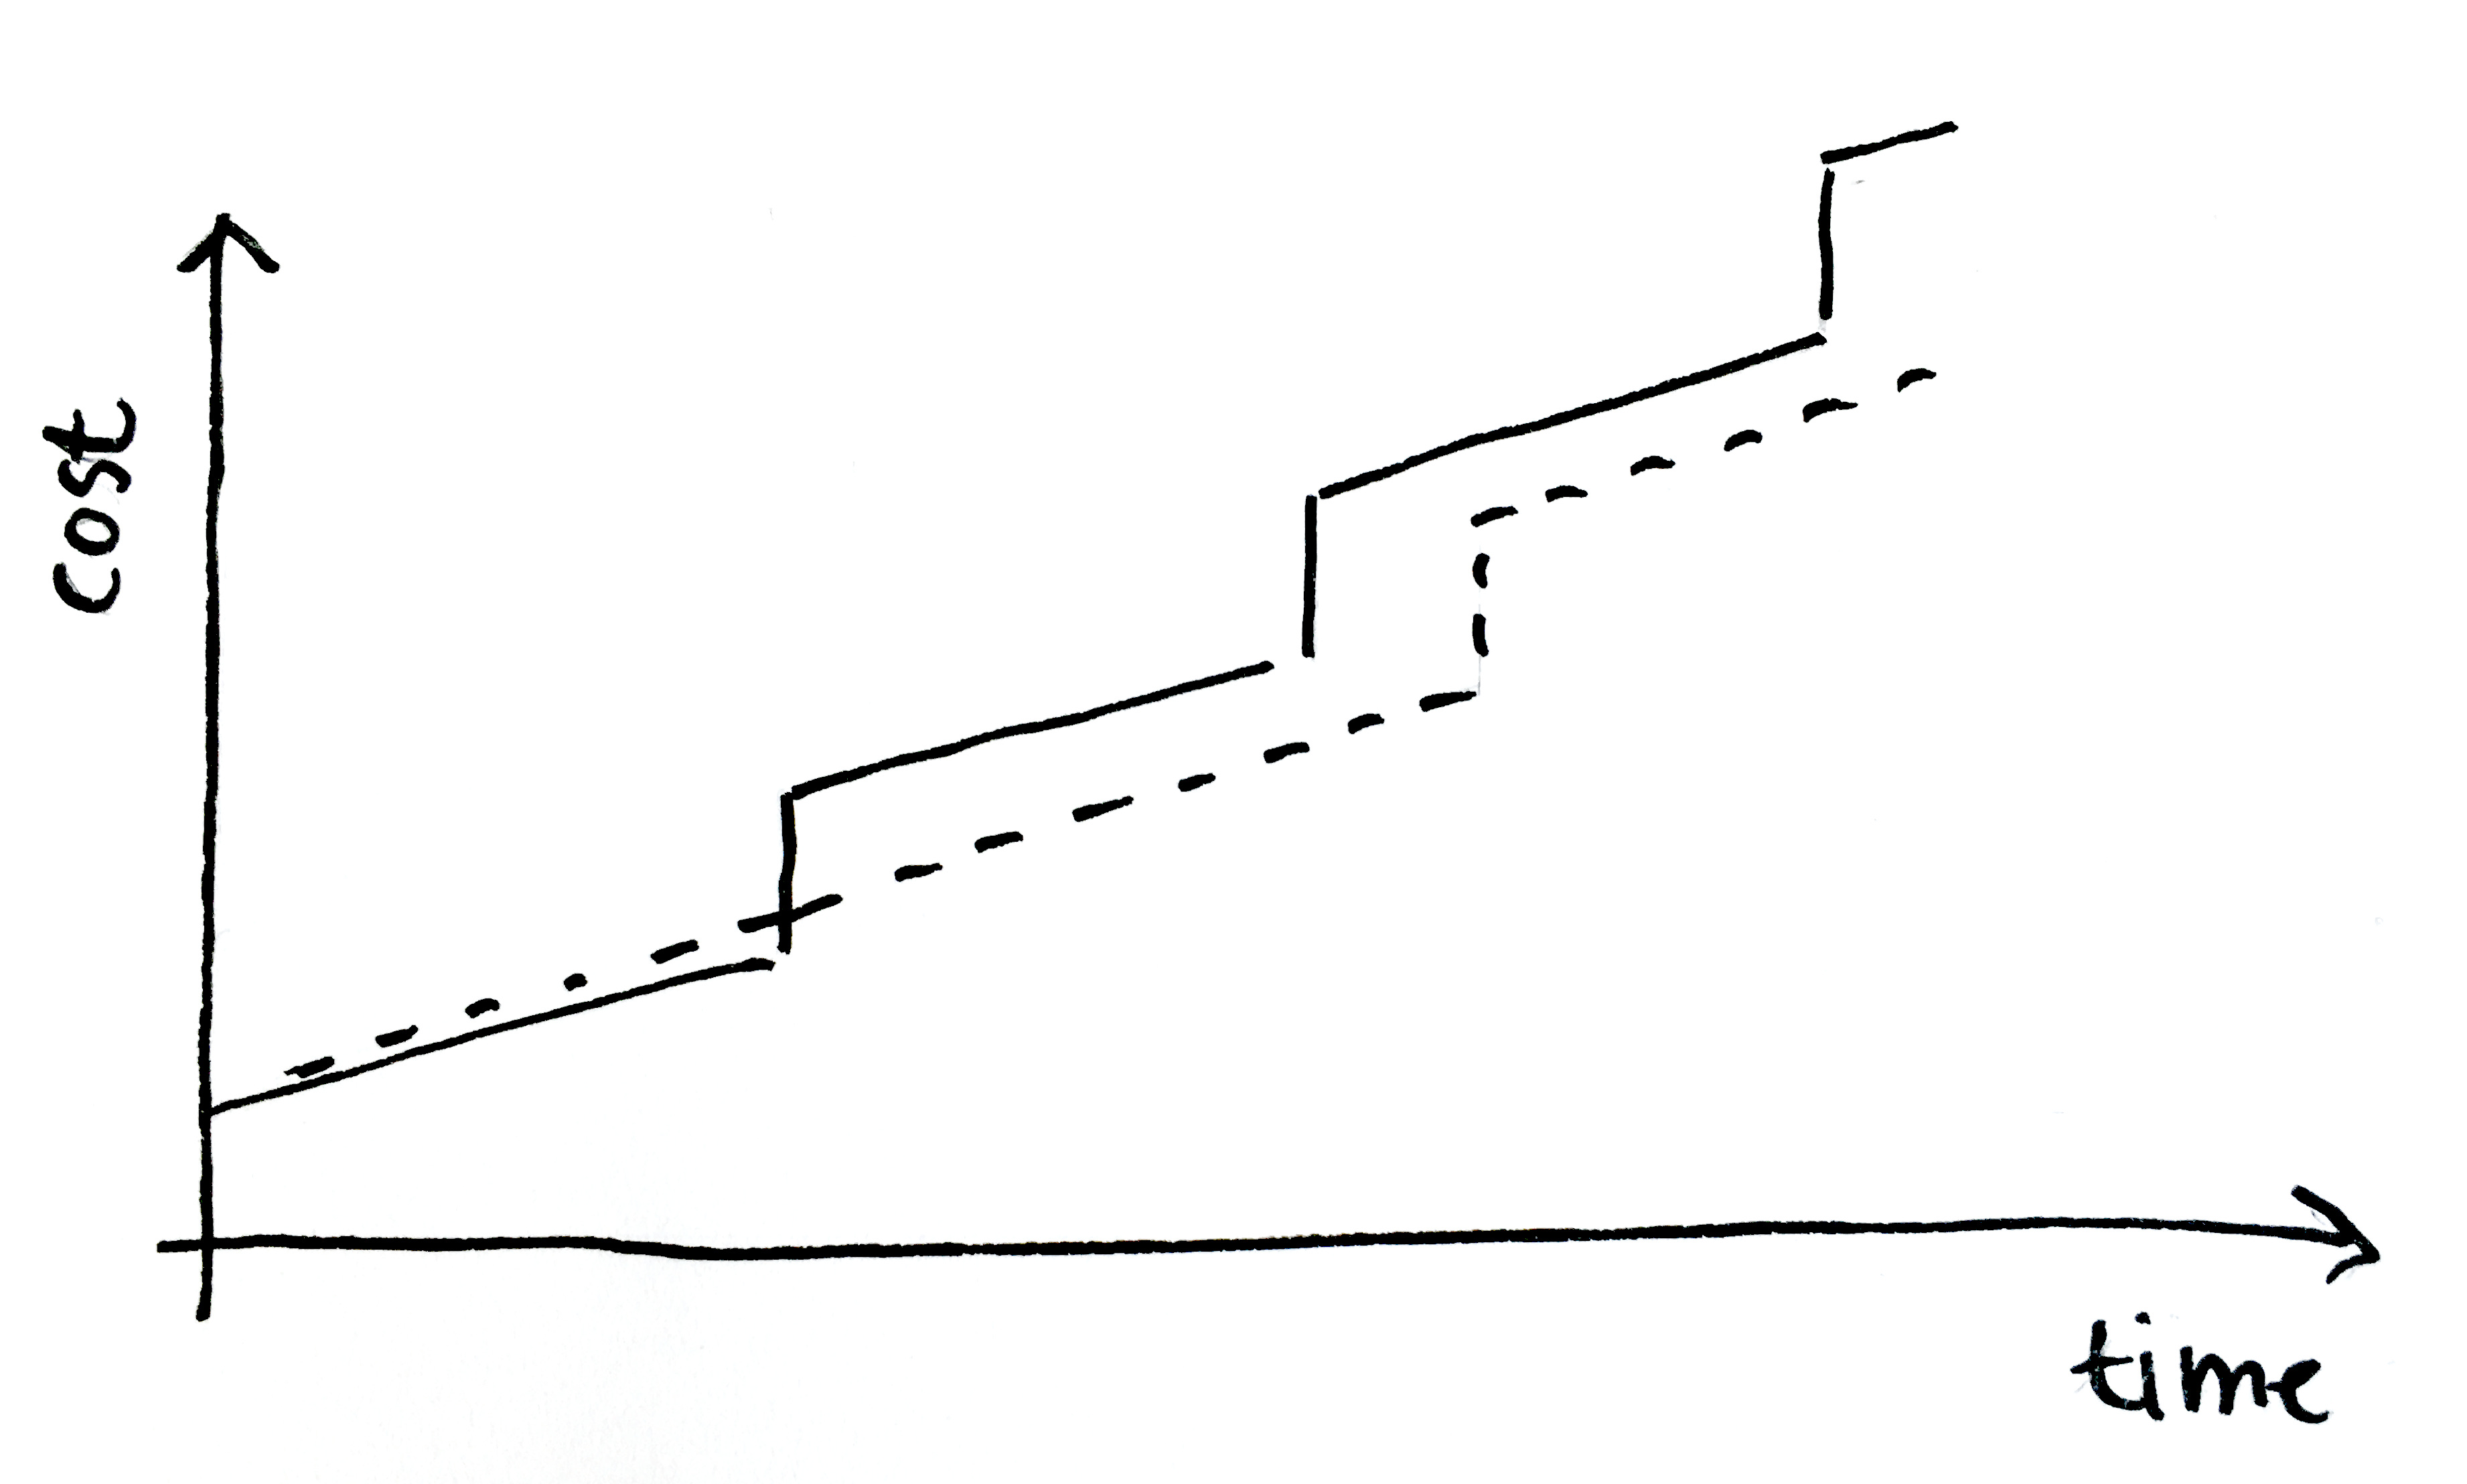
\includegraphics[width=8cm]{img/hypothesis.jpg}
\end{figure} 


\section{Data}

In this experiment only synthetic data will be used. The choice is both practical and a methodologically motivated. First, the production system cannot be altered in such a way that real world data could be tapped within this experiments ,timeframe. Also, real world data in this system differs from one time period to another both in terms of the highscore distribution and throughput -- and of course, data from one application differs from data from other applications. Using synthetic data make the results more general.

\todo{Something about the data used in test}

\todo{Same random seed is always used}

\section{What and how to measure}

To be able to test the hypothesis relative error and execution time will be logged per ranking request.

For the \emph{true} value for calculating the relative error, an exact rank is calculated for that instant. While using other values as true values, such as values created with a fresh bucket-table every time, the exact value seemed to be the most predictable option.

The execution time is measured by calls to \texttt{System.currentTimeInMillis()} in the servlet receiving the ranking request.

\section{The experiment}

The experiment is implemented in a client-server-model where the client simulate playing a game and sends highscores to the server. The server responds with an estimated rank and the execution time for processing the request. The client is a regular Java program with no bells and whistles and the server consists of a number of servlets designed to run on Google App Engine. 

The test environment is set up by resetting or generating the 100 000 highscore entries with random highscores. Lower number means higher score. The highscores have a Gaussian distribution which is somewhat similar to the distribution of real-world highscores\footnote{The real world highscores are similarly distributed to each other and somewhat similar to a Gaussian distribution. However, no effort has ben made to do a statistical analysis of them.}

\todo{Be more precise about the distribution}

When the client has finnished ``playing'' a round it always get a new highscore. The new highscore is better than the old one by a number drawn from a uniform pseudorandom distribution $1-1000$.

To be able to measure the relative error of the estimates the client starts by asking for a list of all highscores. When the client sends a new highscore to the server it also updates its local highscore list. When the server responds with the rank estimate for the new score, that estimate is compared with the real rank and ultimately used for calculating the relative error.

The type of ranking algorithm to use is set before starting the test.

\subsection{Technical details}

The Companys original implementation of the ranking algorithm is written in Java and runs on Google App Engine and. So is this experiment. This is an overly complicated infrastructure to perform the experiments in as the same results could have been gained with a simple command-line interface application not communicating over HTTP at all. The choice is motivated by the initial ambitions that were a lot higher than the actual outcome.

\subsubsection{Libraries}

A few libraries are used; \emph{Objectify} which provides means for persisting Java objects to the App Engines Datastore
and \emph{Jackson} for parsing and generating JSON-data. Naturally, the App Engine SDK is also used.

\todo{Make list and references}

\section{Limitations}

\todo{The real world data set grows over time. Will be ignored, only focus on case when the set of highscores are reasonably large.}

\todo{Only tested on development server}

\chapter{\label{ranking-algorithms}Ranking algorithms}

\section{What problem do a ranking algorithm solve?}

The main purpose of the algorithms discussed below in this section is to answer the question \emph{Given a score, what is the rank of a user or item with this score?} \cite{codejam}. The opposite question -- \emph{Given a rank, what is the score for this rank?} is very similar but not adressed here directly even though most approaches to the ranking problem indirectly answers that question too.

\todo{How to be more formal about this?}

\section{\label{definition}What is ranking?}

\begin{shaded}
  
  What is ranking, formal definition
 
The rank of a well-founded set is defined inductively as the smallest ordinal number greater than the ranks of all members of the set.[1] In particular, the rank of the empty set is zero, and every ordinal has a rank equal to itself.
\href{https://en.wikipedia.org/wiki/Von\_Neumann\_universe}{Wikipedia - Von Neumann universe}

Well founded relation:

$\forall S \subseteq X ( S \neq \varnothing \rightarrow \exists m \in S \forall s \in S (s, m) \notin R)$ \href{https://en.wikipedia.org/wiki/Well-founded\_relation}{Wikipedia - Well-founded relation}

Define ordinal (each ordinal is the well-ordered set of all smaller ordinals?)

\end{shaded}

\subsection{Types of ranking algorithms}

Ranking algorithms can coarsely be divided in two categories: \emph{exact} and \emph{approximating} algorithms. The exact algorithms deal with the ranking problem by sorting and counting. The sorting part is commonly accomplished by indexing the score-property of the entity or the corresponding column in a table in case a relational database is used.  

As mentioned in the introduction, obtaining an exact rank may not be necessary. Other considerations such as speed and cost may be more important. Approximating algorithms estimate the rank by linear interpolation within a segement of ranks. Suitable segments can be found with an \emph{offline-method} such as scanning all scores periodically keeping track of scores at the segments boundaries (See section \ref{bucket}) or with an \emph{online-method} with a \emph{streaming algorithm} that maintains a model for estimating ranks by continuosly updating a number of statistical measures.

\subsubsection{Stability}

In both cases a sorted list needs to be created. If the chosen sorting algorithm is not stable the ranking will be non-deterministic. This may or may not be a problem depending on the application. 

\todo{Strategies as in \href{https://en.wikipedia.org/wiki/Ranking\#Strategies\_for\_assigning\_rankings}{Ranking (Wikipedia)}?}

\section{Exact algorithms}

\subsection{Rank by counting}

From the \hyperref[definition]{definition of ranking} we can quite simply arrive in a solution for obtaining the rank for a score. This would be the naive solution -- getting the rank by counting the number number of highscores greater than the score in question.

This way of getting the rank can be done with a simple query in SQL
\texttt{SELECT count(id) FROM Highscores WHERE Score > TheScore} or by increasing a counter while iterating through an ordered set of highscores in case a non-relational database is used. In any case the items should be indexed on the highscore-field.

Nevertheless, obtaining rank for a score by this method implies scanning through all items having a score higher than the one you want to obtain the rank for. The time complexity of this approach is obviously $\mathcal{O}(n)$ making it unusable for online applications in terms of cost and response time\footnote{If the ranking function is not required to return a new rank, the actual rank could be assigned periodically by a background job to all the highscores. In this case the $\mathcal{O}(n)$ time complexity would be more tolerable.}.

\iffalse
\begin{shaded}

 \emph{I want to define ranking by counting like this:}

  1. define a set of items, and an item i with score s.

  2. define a sorted list of those items or someway indicate that the set is sorted by some relation

\textbf{either}
  
  3a. assign ordinal numbers to the items \\
  4a. get the ordinal number for the i.

 \textbf{or}

  3b. count items before i

\textbf{or}

  3c. Better way of counting items ``before'' the new item?
  
\end{shaded}
\fi

\subsection{Tree based approach}

As described above, ranking is fundamentally a counting problem. One way to accomplish counting more efficiently is by storing the count of each score in an N-ary tree. Each non-leaf node defines a score range and its associated count and the leaves represents individual items from the value domain, ie discreete scores.

Score updates and getting the rank for a score with this algorithm has a time complexity of $\mathcal{O}(\log{} n)$. Since fetching or updating a node may be relatively expensive in case it has to be fetched from a database system the number of ranges per node needs to be chosen so that the height of the tree remains reasonable low\footnote{The Google Code Jam Ranking Library uses 100 buckets per node}. The height of the tree is $ceil(log_{rangesize}numscores)$.

There are a number of things to consider with this approach. First, to get exact rankings the trees leaf nodes need to have as many children as there are possible scores. One way to get around that problem could be to not store individual scores but ranges. This could be done in at least two ways; by defining the ranges in beforehand or by compressing the tree at some interval so that if a childs score range has only a small frequency of its scores, then just dont build the tree further from that child. This is essentially the solution proposed by Shrivastava et al\cite{quantile_digest} with their Quantile Digest algorithm. The solution would then not be able to give exact ranks for scores.

Also, the the score distribution need to be known or the tree need to adapt to the changing score distribution over time to get an optimal solution.

\begin{figure}[h!]
  \centering
  \caption{Example of how ranking is done using a tree-based approach. To get the rank for score 30, start by adding the counts for scores greater than 30. There is 22 higher scores and rank for score 30 is thus 23.\\This figure is a reproduction of a similar image from the article \emph{Fast and Reliable Ranking in Datastore} \cite{ranking-in-datastore} 
 , licensed under the Creative Commons Attribution 3.0 License}   \label{fig:tree}
\hbox{\hspace{-0.8cm}
  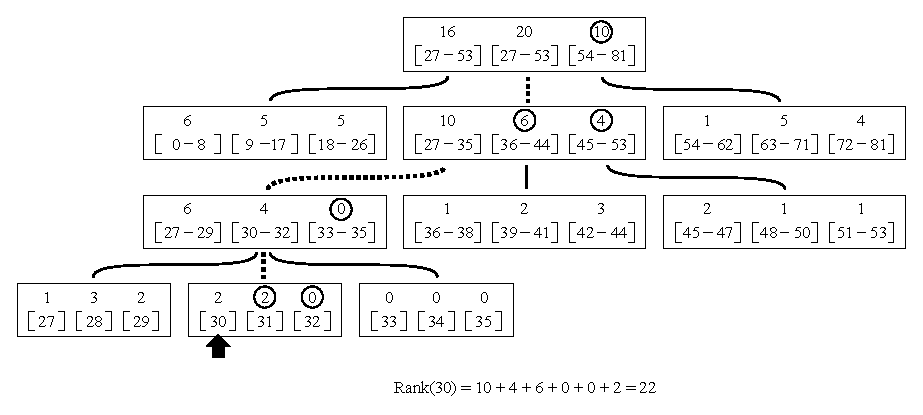
\includegraphics[width=15cm]{img/tree.eps}}
\end{figure}

\section{Approximating algorithms}

Getting an exakt rank for a score may not be crucial. One fairly obvious class of solutions is the ones using linear interpolation of rank within a score range with known ranks at the boundaries. The ranks and score ranges needed for the interpolation may be acquired in different ways of which two will be described in this chapter; Buckets with Global Query and Frugal Streaming.

\subsection{How to measure error}

Approximating algorithms will almost by definition deviate from the \emph{true value} and we need a way to express that deviation. 
One way could be expressing the error in absolute terms as \ref{abs-error}.
\begin{equation}
  \label{abs-error}
  \varepsilon_{abs} = x - x_0 = \Delta x
  \end{equation}

Another option would be expressing the error as the \emph{relative error}, defined by \href{http://mathworld.wolfram.com/RelativeError.html}{mathworld.wolfram.com}
as \ref{rel-error}.

\begin{equation}
  \label{rel-error}
  \delta x = \frac{\Delta x}{x} = \frac{x_0 - x}{x} = \frac{x_0}{x} - 1
\end{equation}

A consequence of measuring the relative error when it comes to ranking is that a small rank estimate error will generate a large error when the estimating a high rank, and a relatively small error when estimating lower ranks with the same ranking error in absolute terms, for example see \ref{e1} and \ref{e2} where $|\Delta x| = 1$ in both cases.

\begin{equation}
  \label{e1}
x_0 = 9, x = 10 \implies \delta x = \frac{9 - 10}{10} = -0.1  
\end{equation}

\begin{equation}
  \label{e2}
x_0 = 999, x = 1000 \implies \delta x = \frac{999 - 1000}{1000} = -0.001  
  \end{equation}


Which way to go is application-dependent, but when talking about ranking highscores in games the relative error is a very practical measure because it fits the real world concerns very well.

\subsection{\label{bucket}Buckets with Global Query}

The most basic way to go with the linear interpolation approach is called \emph{Bucket with Global Query} in the article \href{https://cloud.google.com/datastore/docs/articles/fast-and-reliable-ranking-in-datastore/}{Fast and Reliable Ranking in Datastore} \cite{ranking-in-datastore}. The same type of algorithm is also in use by the company mentioned in the introduction.

A background job periodically scans all highscores, creating a table with entries for scores and corresponding ranks. An excerpt from the created bucket-table may look like table \ref{table:ranking-table}. So, for example, to estimate the rank for score $2\;050$ which falls in bucket 6, start by calculating what the score range in bucket 6 is, in this case $2\;204 - 1\;961 = 243$. $2\;050$ is $89$ scorepoints ``in'' the bucket and hence the rank is calculated as $83 + 23 \times \frac{89}{243} \approx 91$. The same calculation is illustrated in figure \ref{fig:linear}.

\begin{figure}[h!]
  \centering
  \caption{Linear interpolation}
  \label{fig:linear}
  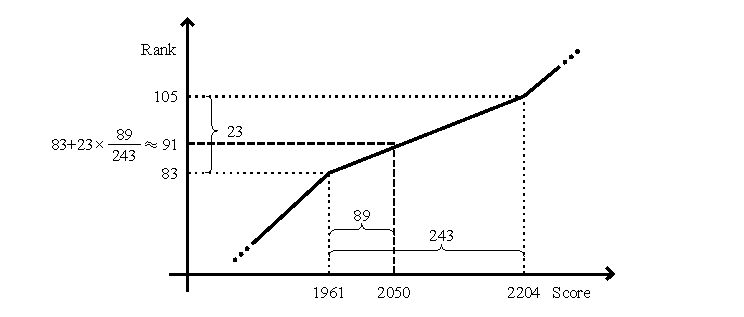
\includegraphics[width=13cm]{img/linear_interpolation.eps}
\end{figure}

\begin{table}[h]
  \begin{center}
  \begin{tabular}{ c c c c }
    Bucket no & Start score & Start rank & Size \\
    5 & 1 515 & 83 & 22 \\ 
    6 & 1 961 & 105 & 23 \\ 
    7 & 2 204 & 128 & 23 \\ 
    8 & 2 574 & 151 & 24 \\  
    9 & 2 852 & 175 & 25 \\ 
  \end{tabular} 
  \caption{Excerpt from bucket-table}
  \label{table:ranking-table}
  \end{center} 
\end{table}

The quality of the estimates made by this method depends on several factors.
\textbf{The frequency of the periodic scans} needs to be high enough to keep the error of the estimate at an acceptable level. Also, \textbf{the size of the buckets} have an impact on the result. Yet another factor that cannot be handled in a simple way is when the score distribution within a bucket are skewed or simply not very linear within the score range as in figure \ref{fig:uneven}.

\begin{figure}[h!]
  \centering
  \caption{An example of an uneven distribution of highscores within a bucket.
    In this case, a score in the middle of the actual distribution in the beginning of bucket a would get a rank estimate based on the score range defined by start scores of bucket a and b, which in this example would result in to a higher rank than the actual.}
  \label{fig:uneven}
  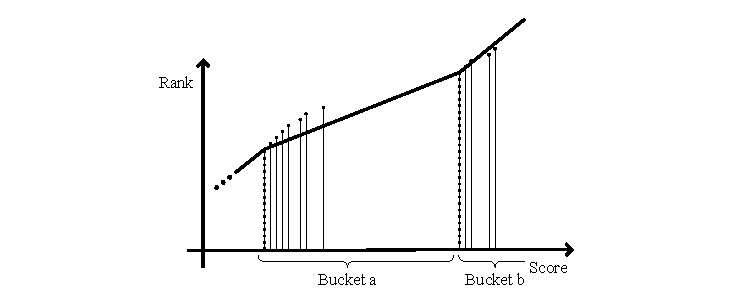
\includegraphics[width=13cm]{img/uneven_distribution.eps}
\end{figure}

If an update of a highscore from a lower score to a higher occurs but the new score is within the the same bucket as the previous score, the subsequent estimate will be the same for any score since the bucket-table is unchanged. Because the underlying distribution is changed the error may be different but not necessarily worse.

\todo{Illustration}
\todo{This is not 100 \% correct}

On the other hand, if a highscore estimate goes from a lower rank bucket to a higher one, a subsequent scan of the highscores would result in a table where the new bucket will grow by one and, start-rank of buckets after the new to and including the former one will increase by one and the bucket for the previous estimate would shrink by one.

\todo{Illustration}

% \begin{figure}[h]
%  \centering
%  \caption{A new highscore breaking the bucket-table}
%  \label{fig:change-buckets}
%  
\includegraphics[width=8cm]{img/change-buckets.png}
%\end{figure}

Future highscore updates will add to the bucket-tables deviation from a theorethical \emph{true} bucket-table and as a consequence the estimates will show a growing error with respect to the true rank until the bucket-table is recreated (Figure \ref{fig:errortime}). It is worth noting that the error should not be expected to be zero even with a fresh bucket-table since estimates is precisely that -- estimates.

\begin{figure}[h]
  \centering
  \caption{Error in estimates will grow over time, until the bucket-table is recreated and the error level drops down to the initial error.
  }
  \label{fig:errortime}
  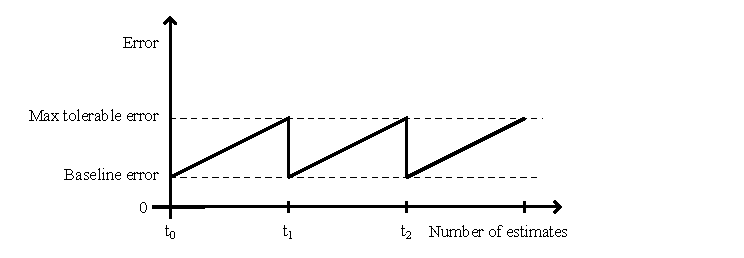
\includegraphics[width=13cm]{img/error-over-time.eps}
\end{figure}

\subsubsection{Handling errors}

A common requirement is that ranking have to be more precise, that is small $\varepsilon_{abs}$, for higher ranks than for lower ranks. This may be accomplished by having small buckets for higher ranks while increasing the bucket size by some formula for the lower ranks as in figure \ref{fig:growing}.  By using this method higher ranks will be predicted with better precision and the bucket-table will stay reasonably small. In some cases even an exponential bucket-growth will produce good enough result for the application.
 
\begin{figure}[h!]
  \centering
  \caption{Growing bucket sizes}
  \label{fig:growing}
  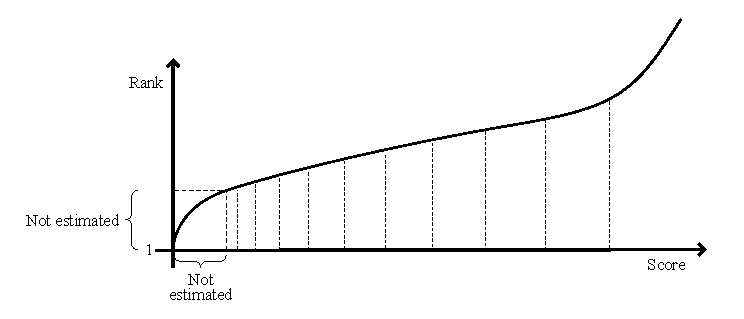
\includegraphics[width=13cm]{img/growing_bucket_sizes.eps}
\end{figure}

However, the method described above may not be enough to handle the highest ranks. One reason for that may simply be that the requirements on the algorithm and ultimately the final solution do not accept approximations \emph{at all} for the top ranks. To solve that problem this algorithm can be paired with the \emph{Rank by counting}-algorithm for the highest ranks. This should not be a problem since  the counting involves only the critical and highest ranks which can easily be fetched if the data is indexed. When to not estimate can be decided by looking at variables such as the score or rank estimate. 

\subsection{Online approaches, streaming algorithms}

\begin{mdframed}[backgroundcolor=red,innerleftmargin=15pt,leftmargin=-10pt,rightmargin=-10pt, innerrightmargin=15pt,innertopmargin=10pt,innerbottommargin=10pt, fontcolor=white, skipabove=20pt, linewidth=0]
  \textbf{Warning! Bumpy road ahead!}
  
  I wish to complete the rest of this chapter for this thesis. It is not essential to my experiments and conclusions later but it provides a completeness to the subject I think would be good.
\end{mdframed}

The drawback with the method described above is that the bucket-table after some time will no longer represent the actual distribution of scores and consequently less and less accurate rankings.

An alternative but still similar way of solving the problem could be by estimating a number of quantiles of the distribution of highscores by using a streaming algorithm. 

\emph{Frugal streaming} is a streaming streaming algorithm for estimating a quantile of a stream devised by Ma, Muthukrishnan and Sandler. \cite{frugal_streaming} The algorithm itself is fairly self explanatory (see appendix \ref{frugal}) and have a small memory footprint.

The idea is that by calculating a number of quantiles for every new highscore while keeping track of the total number of highscores you could create a bucket-table as in the algorithm described in section \ref{bucket}.

Calculating exact quantiles of a large dataset is quite expensive.

\subsection{Quantile Digest}

\emph{Quantile Digest} is a tree based stream summary algorithm. The paper that describes the algorithm does it from a sensor network perspective 
The algorithm builds a binary tree of the value domain. The tree is then compressed and can be sent to the parent of the sensor. The compression is lossy such that less frequent values are represented as a bucket. The result of the compression is called Quantile Digest.

Quantile query - inverse quantile

\blockquote{

Inverse Quantile: Given a value x, determine its
rank in the sorted sequence of the input values.
175
In this case, we again make the same sorted list (L),
and traverse it from beginning to end. We report the
sum of counts of buckets $v$ for which $x > v.max$ as
the rank of x. The reported rank is between rank(x)
and rank(x) + $\varepsilon$, $rank(x)$ being the actual rank of
$x$.}

\chapter{Result}

\begin{shaded}
  Describe results
  \end{shaded}

\chapter{Conclusion and Future Directions}

From the results in the previous chapter it is clear (somewhat clear) that the improved ranking algorithm with dynamic buckets perform better with the current settings of the experiment.

There are however a bunch of parameters to play with in both cases, such as initial bucket sizes when it comes to tuning the algorithm itself and the distribution of the initial highscores as well as the distribution of the highscores generated during the test.

There are at least two interesting paths to follow from here. First, the Company do not have a clear definition of what good enough ranking is. Their current rank estimates are obviously good enough but maybe even unnecessarily good with too frequent rebuilds of the bucket table. Secondly, optimizing the new implementation by utilizing a memory cache on a lower level would probably result in significant gains.





\cleardoublepage

\addcontentsline{toc}{chapter}{\bibname}
\bibliographystyle{plain}
\bibliography{sources}

\appendix

\chapter{\label{frugal-alg}Frugal streaming}


\section*{Algorithm Frugal-1U}

Input: Data stream $S$, $h$, $k$, 1 unit of memory $m$.

Output: $m$

$m = 0$\\
for each $s_i$ in $S$ do \\
\hspace*{5mm}$rand$ = random(0,1) \\
\hspace*{5mm}if $s_{i} > m$ and $rand > 1 - \frac{h}{k}$ then\\
 \hspace*{10mm}    $m = m + 1$ \\
\hspace*{5mm}  else if $s_{i} < m$ and $rand > \frac{h}{k}$ then\\
\hspace*{10mm}     $m = m - 1$ \\
\hspace*{5mm}end if\\
end for\\


 


\chapter{Source code}

\href{https://github.com/carlevert/bt}{GitHub}


% \chapter{First Appendix}

\end{document}
 
